\documentclass{article}

\usepackage[T1]{fontenc}
\usepackage[
  letterpaper,
  top=2cm,
  bottom=2cm,
  left=3cm,
  right=3cm,
  marginparwidth=1.75cm
]{geometry}
\usepackage{amsmath,amssymb}
\usepackage{booktabs}
\usepackage{tabularx}
\usepackage{graphicx}
\usepackage[section]{placeins}
\usepackage{microtype}
\usepackage{xcolor}
\usepackage{xspace}
\usepackage[colorlinks=true,allcolors=blue]{hyperref}
\graphicspath{{assets/}}

% Keep figure-only pages top aligned instead of vertically centering short panels.
\makeatletter
\setlength{\@fptop}{0pt}
\makeatother

% Portable bold mathematics for the repository-local minimal TeX bundle.
\renewcommand{\boldsymbol}[1]{\pmb{#1}}
\DeclareMathSizes{10}{10}{7}{6}
\DeclareFontFamily{T1}{lmrbm}{}
\DeclareFontShape{T1}{lmrbm}{bx}{n}{<-> ec-lmbx10}{}
\SetMathAlphabet{\mathbf}{normal}{T1}{lmrbm}{bx}{n}

\newcommand{\method}{EFF-Dock\xspace}
\newcommand{\angstrom}{\text{\normalfont\AA}}
\newcommand{\R}{\mathbb{R}}
\newcommand{\SO}{\mathrm{SO}}
\newcommand{\SE}{\mathrm{SE}}
\newcommand{\citep}[1]{\cite{#1}}
\newcommand{\sisection}[1]{\href{SI.pdf}{Supplementary Information, Sec.~#1}}

\title{\method: Fragment-Based \(\SE(3)\)-Equivariant Flow Matching\\
for Protein--Ligand Docking}
\author{\parbox{0.96\textwidth}{\centering
Jaemin Sim\textsuperscript{1} and Juyong Lee\textsuperscript{1,2,3,4,*}\\[0.75em]
\small\textsuperscript{1}Department of Molecular Medicine and Biopharmaceutical Sciences, Graduate School of Convergence Science and Technology, Seoul National University, Seoul 08826, Republic of Korea\\
\small\textsuperscript{2}College of Pharmacy, Seoul National University, Seoul 08826, Republic of Korea\\
\small\textsuperscript{3}Research Institute of Pharmaceutical Science, College of Pharmacy, Seoul National University, Seoul 08826, Republic of Korea\\
\small\textsuperscript{4}Arontier Co., Seoul 06735, Republic of Korea\\[0.5em]
\small\textsuperscript{*}Corresponding author: \href{mailto:nicole23@snu.ac.kr}{nicole23@snu.ac.kr}
}}
\date{}

\begin{document}
\maketitle

\begin{abstract}
Protein--ligand docking requires accurate candidate generation, physically plausible coordinates and reliable pose selection. We present \method, a fixed-receptor, supplied-pocket method that learns a flow over the translations and rotations of rigid ligand fragments. An equivariant protein--ligand graph network predicts atom-wise vectors that are projected onto fragment motion, a separate network ranks candidates, and a differentiable interaction energy refines their geometry. Across five reference-pocket redocking cohorts, refined 100-pose banks contained a candidate with RMSD below \(2\,\angstrom\) for 87.9--96.5\% of complexes. Refinement followed by rescoring increased selected-pose RMSD--PoseBusters success by 15.7--23.2 percentage points under the primary chirality-filtered selector (21.7--26.5 without filtering), giving success rates of 53.2--80.0\%. In 12.4--34.4\% of complexes, the eligible bank contained an RMSD-successful candidate but the selected pose was not RMSD-successful. These analyses distinguish candidate availability, coordinate validity and ranking loss, while pocket-center perturbations expose generation-input sensitivity with fixed downstream spatial context.
\end{abstract}

\label{sec:introduction}

The three-dimensional pose of a small molecule determines its protein contacts and shapes subsequent structure--activity analysis.
Experimental complexes provide the best reference, but they are unavailable for many targets and ligand series.
Protein--ligand docking fills this gap by predicting ligand placement and conformation for a prepared receptor.
Here we study fixed-receptor docking with a supplied binding site; pocket discovery, binding classification, and affinity prediction are outside the scope of the model.

Docking remains difficult because global placement and internal conformation are coupled on a rugged, multimodal landscape.
A finite search must resolve translation, orientation, rotatable bonds, covalent geometry, and local protein--ligand complementarity.
Protonation and tautomeric state, cofactors, metals, solvent, and receptor reorganization create additional ambiguity that is not removed by increasing the number of sampled poses.
Classical docking programs combine conformational search with approximate scoring \citep{trott2010vina,eberhardt2021vina}.
GNINA augments this workflow with learned three-dimensional convolutional scoring \citep{mcnutt2025gnina}.
Their output depends strongly on receptor preparation, search-region definition, flexibility settings, and post-docking refinement.

Learned geometric models have broadened both the search mechanism and the task definition.
DiffDock samples ligand translation, rotation, and torsion by a diffusion process \citep{corso2023diffdock}; Uni-Mol Docking V2 predicts poses within a specified binding pocket \citep{alcaide2024unimoldocking}; and DiffBindFR jointly treats ligand motion and selected receptor-side-chain flexibility \citep{zhu2024diffbindfr}.
DynamicBind generates ligand-specific receptor conformations \citep{lu2024dynamicbind}, FlowDock applies conditional geometric flow matching to flexible complex generation \citep{morehead2025flowdock}, and AlphaFold~3 addresses a broader biomolecular cofolding problem \citep{abramson2024alphafold3}.
These methods solve different tasks and receive different receptor and pocket information.
Direct docking comparisons use supplied-pocket protocols and retain each method's native receptor handling; benchmark-specific comparisons additionally report cofolding results with their different input conditions specified.

A docking pipeline has three main components: pose generation, candidate ranking, and coordinate validation.
Oracle minimum RMSD over a finite candidate set measures sampling coverage, not top-1 docking.
A low ligand RMSD also does not guarantee valid stereochemistry, bond geometry, or protein--ligand contacts \citep{buttenschoen2024posebusters}.
We report coverage, selected top-1 accuracy, PoseBusters validity, and RMSD--PoseBusters success as separate endpoints.
A confidence network is used only for ranking within a candidate bank, consistent with recent work that separates pose quality from binding-oriented predictions \citep{sim2026rmsdpred}.

Ligand flexibility can be parameterized at several geometric scales.
Treating the ligand as one rigid body preserves internal geometry but cannot represent torsional rearrangement.
Direct all-atom generation is flexible but requires the model to maintain covalent structure while solving global placement.
Torsion-tree methods preserve local bond geometry, although each rotation moves a convention-dependent downstream subgraph.
Classical incremental docking instead anchors and grows rigid ligand pieces \citep{rarey1996incremental}, while chemistry-oriented schemes such as Breaking of Retrosynthetically Interesting Chemical Substructures (BRICS) define fragments for a different purpose: retrosynthetically meaningful molecular decomposition \citep{degen2008brics}.
SigmaDock applies diffusion to rigid-fragment ligand poses \citep{prat2025sigmadock}.
Our decomposition cuts a restricted set of rotatable bonds to define rigid components that move simultaneously.
It lies between a single rigid ligand and unconstrained atom coordinates, while soft geometric terms maintain the cut interfaces.

Flow matching learns a continuous vector field that transports a tractable prior toward a data distribution without integrating the generative ordinary differential equation (ODE) during training \citep{lipman2023flow}.
Its extension to non-Euclidean state spaces provides a natural language for translation--rotation products \citep{chen2024generalgeometries}. Matcha applies multistage Riemannian flow matching to molecular docking \citep{frolova2026matcha}.
Equivariant tensor-product networks allow scalar, vector, and higher-order features to transform consistently under a joint rigid motion \citep{liao2023equiformer}.
Related flexible-docking work has used Newton--Euler mechanics to map interaction energy to geometric motion \citep{huang2024redock}.
In \method, a shared protein--ligand network instead predicts atom-level equivariant vectors and aggregates them for each ligand fragment.
An independently parameterized interaction energy provides pose diagnostics, optional inference guidance, and post-sampling refinement.

\method represents the ligand on a product of fragment rigid-body pose spaces.
A heterogeneous graph connects ligand atoms and fragments with protein atoms and residue nodes through covalent, topological, and spatial relations.
A shared \(\SE(3)\)-equivariant trunk and fragment-wise Newton--Euler readout define the conditional flow, while a separate confidence model ranks the sampled poses.

Here we evaluate candidate availability, physical validity and pose selection separately across five reference-pocket redocking cohorts. The experiments assess the resulting pipeline rather than isolating the causal contribution of each architectural component.

\FloatBarrier

\section{Results}
\label{sec:results}

\subsection{Fragment-space docking pipeline}

\method represents a ligand as rigid components obtained by cutting a restricted set of rotatable bonds. A heterogeneous protein--ligand graph conditions a flow over the fragments' translations and rotations (Fig.~\ref{fig:workflow-overview}). An equivariant network predicts one vector per ligand atom; a least-squares rigid-motion projection converts these vectors to fragment velocities (Fig.~\ref{fig:model-architecture}). A separate network predicts a within-bank pose-ranking score. Generated candidates are refined by bounded descent on a differentiable geometric interaction energy and then ranked again. The energy supplies coordinate gradients independently of the learned vector field; it is neither an affinity predictor nor a free-energy model.

The evaluation uses a fixed holo receptor, a reference-derived pocket, 100 candidates and ten integration steps. Three inference repeats use the same docking and confidence weights. The evaluated coordinate-to-feature conventions and their differences from training are specified in Online Methods and Supplementary Information, Secs.~S1.2--S1.3.

\begin{figure}[!htbp]
    \centering
    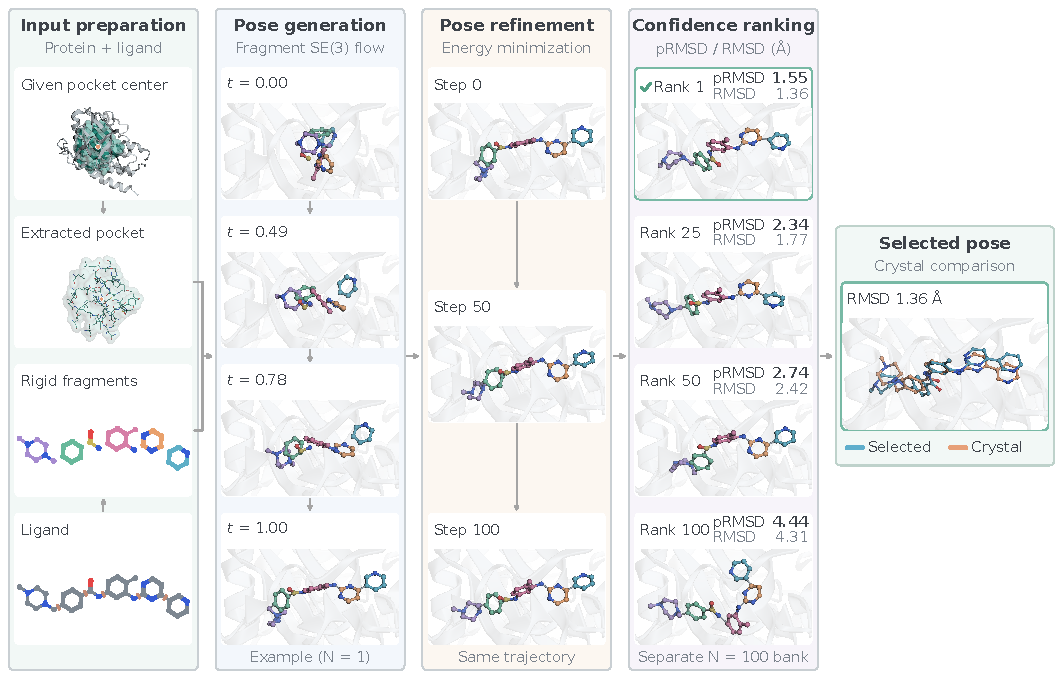
\includegraphics[width=\linewidth,height=0.82\textheight,keepaspectratio]{Fig1.pdf}
    \caption{\textbf{Overview of the \method docking pipeline.} A prepared receptor, one ligand chemical state and conformer, and a supplied pocket center define the input. The ligand is decomposed into rigid fragments whose \(\SE(3)\) states are transported by the learned flow. The illustrated candidate is subsequently optimized by bounded rigid-fragment energy refinement. A separate 100-pose benchmark bank prepared from SMILES is scored by the confidence model, and the selected pose is compared with the crystal pose only for evaluation. The checkmark identifies the selected candidate; crosses mark unselected examples. Candidate ranks use predicted RMSD (pRMSD); the displayed RMSD values are retrospective errors and do not enter selection. The illustrated trajectory uses a supplied starting conformer and is a prespecified one-pose example, not an aggregate benchmark result.}
    \label{fig:workflow-overview}
\end{figure}

\begin{figure}[p]
    \centering
    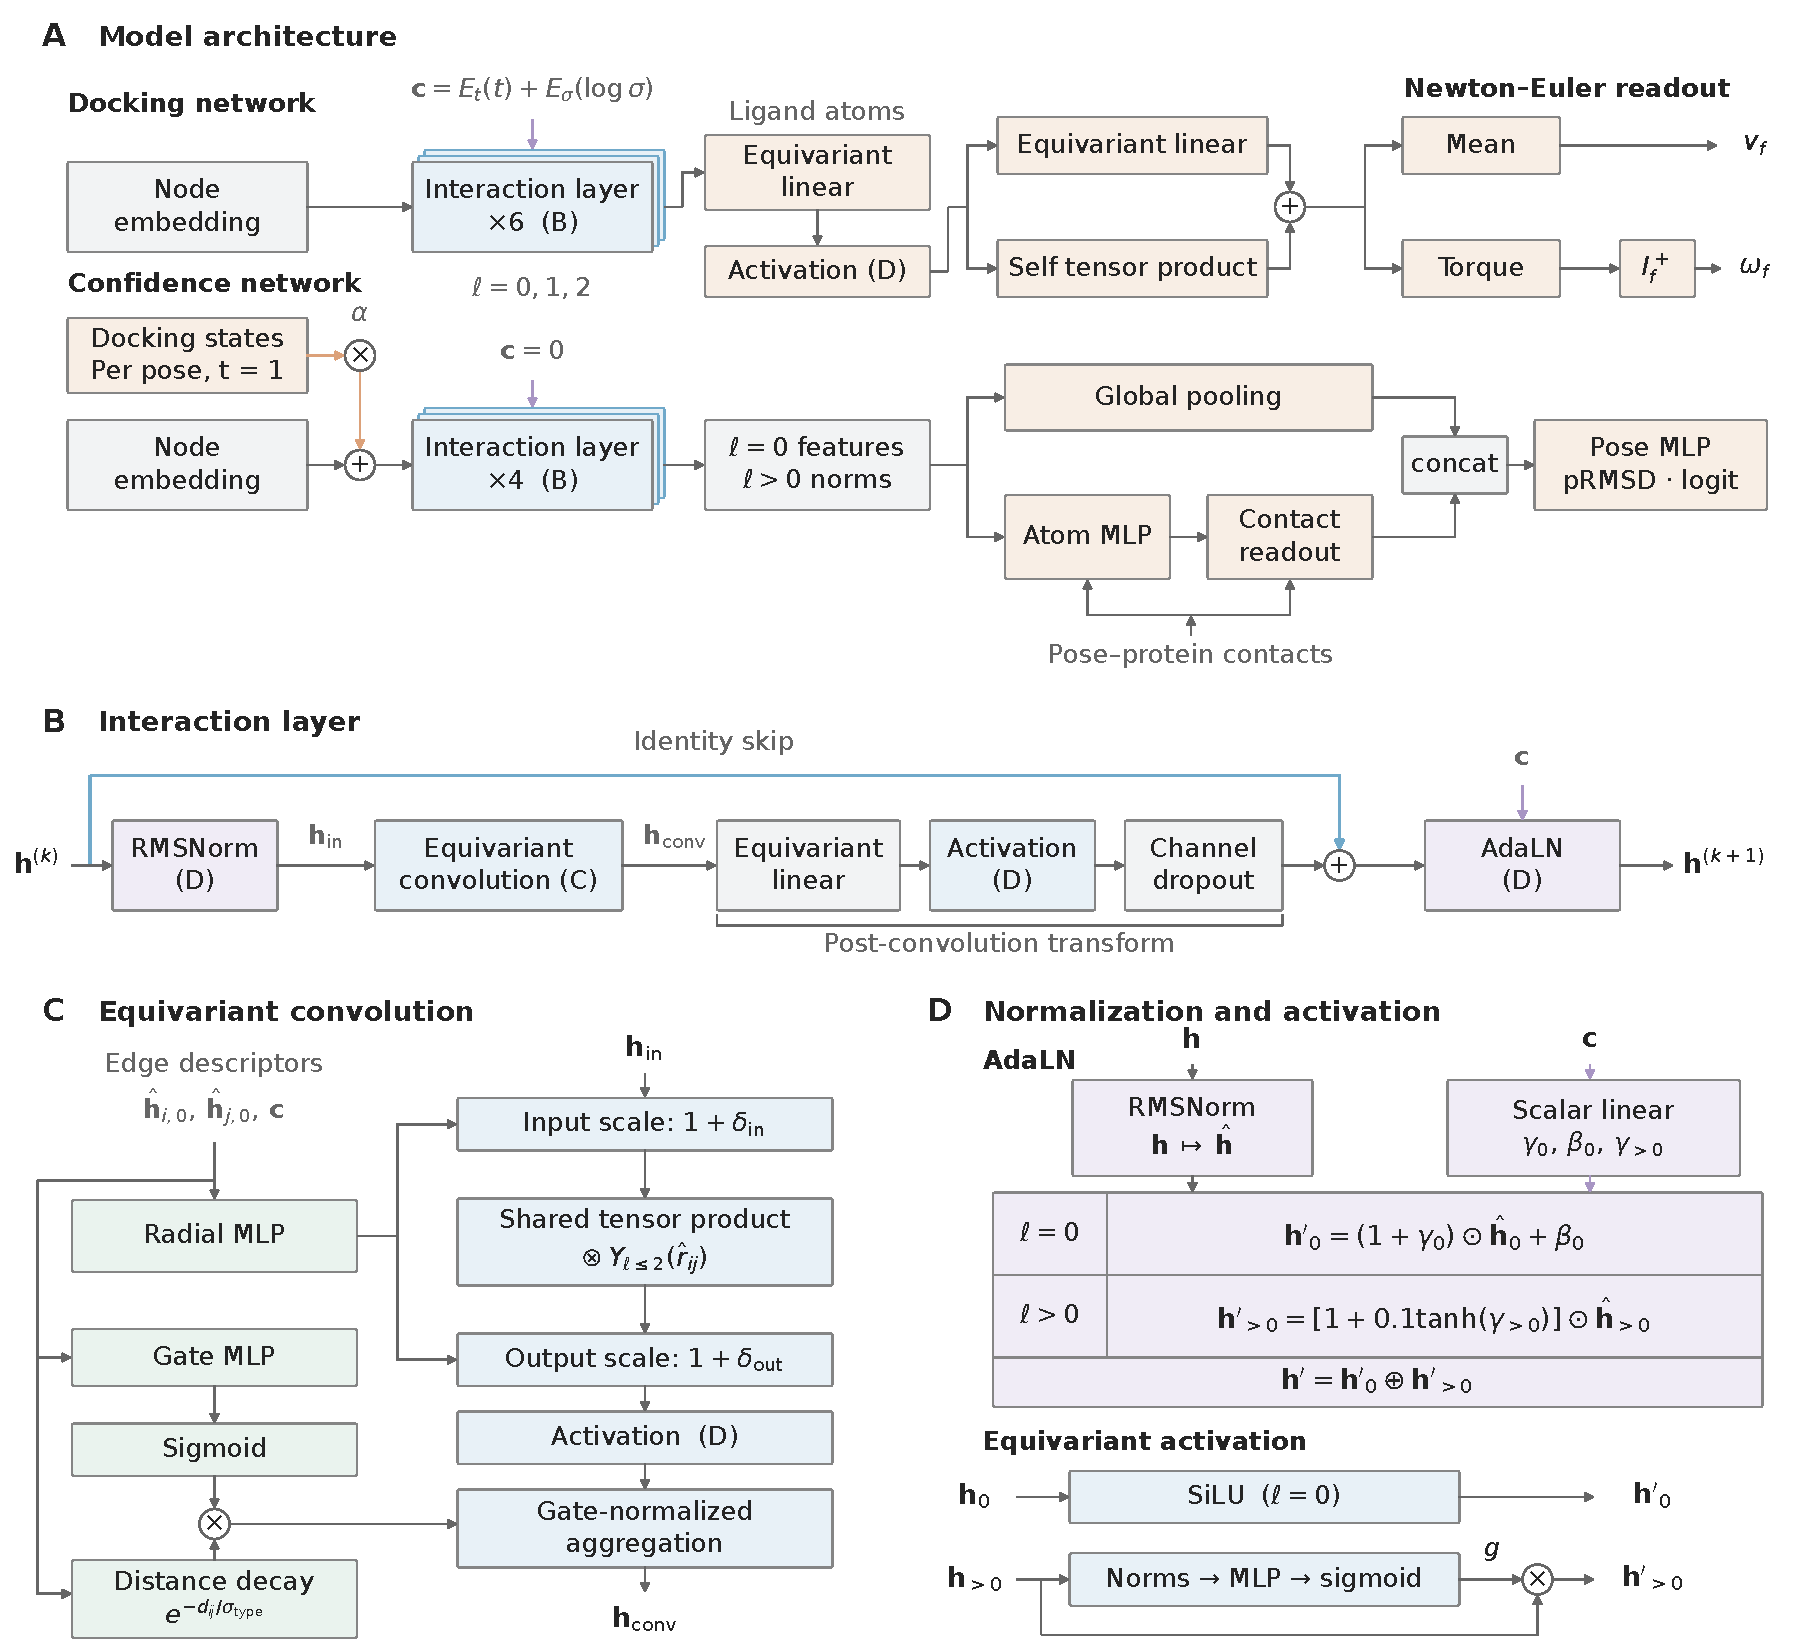
\includegraphics[width=\linewidth,height=0.88\textheight,keepaspectratio]{Fig2.pdf}
    \caption{\textbf{Docking and confidence architectures.} (A) The docking network applies six conditioned equivariant interaction layers and converts ligand-atom features to fragment translation and angular velocities with the Newton--Euler readout. For each candidate, terminal docking features are recomputed at \(t=1\) with its source prior scale. The confidence network combines these with a new embedding, applies four interaction layers with zero conditioning vector \(c=0\), invariantizes the resulting features, and predicts pose-level RMSD and success scores from global and contact-aware summaries. (B) Each interaction layer contains normalization, equivariant convolution, post-convolution transformation, a residual connection, and adaptive layer normalization. (C) The equivariant convolution uses radial and gating networks, shared tensor products through \(\ell\le2\), distance decay, and gate-normalized aggregation with invariant nonscalar rescaling. (D) Scalar and nonscalar channels use type-appropriate adaptive normalization and equivariant activation. Detailed tensor definitions are provided in Supplementary Information, Sec.~S3.}
    \label{fig:model-architecture}
\end{figure}

\FloatBarrier

\subsection{Supplied-pocket comparison}

Fig.~\ref{fig:benchmark-comparison} compares selected-pose RMSD success and RMSD--PoseBusters success on Astex Diverse and PoseBusters v2.
The local comparison includes SigmaDock \citep{prat2025sigmadock}, DiffDock-Pocket \citep{plainer2023diffdockpocket}, RLDiff RL++ \citep{broster2026rldiff}, DiffBindFR \citep{zhu2024diffbindfr}, and force-optimized SurfDock \citep{cao2025surfdock}.
On Astex, EFF-Dock achieved 80.0\% same-pose RMSD--PoseBusters success.
SigmaDock, SurfDock and RLDiff RL++ had higher point estimates on both endpoints.
On PoseBusters v2, EFF-Dock reached 79.1\% RMSD--PoseBusters success. Relative to SigmaDock, the paired difference in RMSD--PoseBusters success was +2.7 percentage points (95\% bootstrap interval, \(-2.3\) to +7.5), compared with \(-9.0\) points (\(-16.1\) to \(-2.0\)) on Astex. The PoseBusters interval does not establish superiority, equivalence or non-inferiority; intervals are unadjusted for multiple comparisons (Supplementary Fig.~S14).
Most selected RMSD-successful EFF-Dock poses also passed PoseBusters.
The learned methods use their native sampling and ranking procedures, while GOLD and Vina are literature values \citep{buttenschoen2024posebusters}; the comparison evaluates protocol-conditioned pipelines with differing receptor and ligand preparation, pocket construction, candidate budgets and native selectors, rather than matched-compute implementations.
Saved-pose reevaluation under benchmark-specific endpoints gave 71.4\% top-1 success on all 558 FoldBench interfaces, requiring BiSyRMSD \(<2\,\angstrom\) and LDDT-PLI \(>0.8\) on the same refined pose. On the official 802-case OpenBind follow-on subset, top-1 BiSyRMSD \(\le2\,\angstrom\) and PoseBusters success was 56.4\%, falling to 48.3\% with the additional LDDT-PLI \(\ge0.8\) requirement (Supplementary Fig.~S20; \sisection{S7.3}). Supplementary Table~S14 compares these results with published cofolding references and GNINA holo redocking, and reports pocket-conditioned PhiBench baselines alongside EFF-Dock top-5 results for 40-pose and 100-pose banks. PhiBench-derived retains the local cohort and fixed-receptor RMSD definition. Task, preparation, evaluability, training exposure and budget differences remain explicit; these comparisons do not establish paired superiority.

\begin{figure}[!htbp]
    \centering
    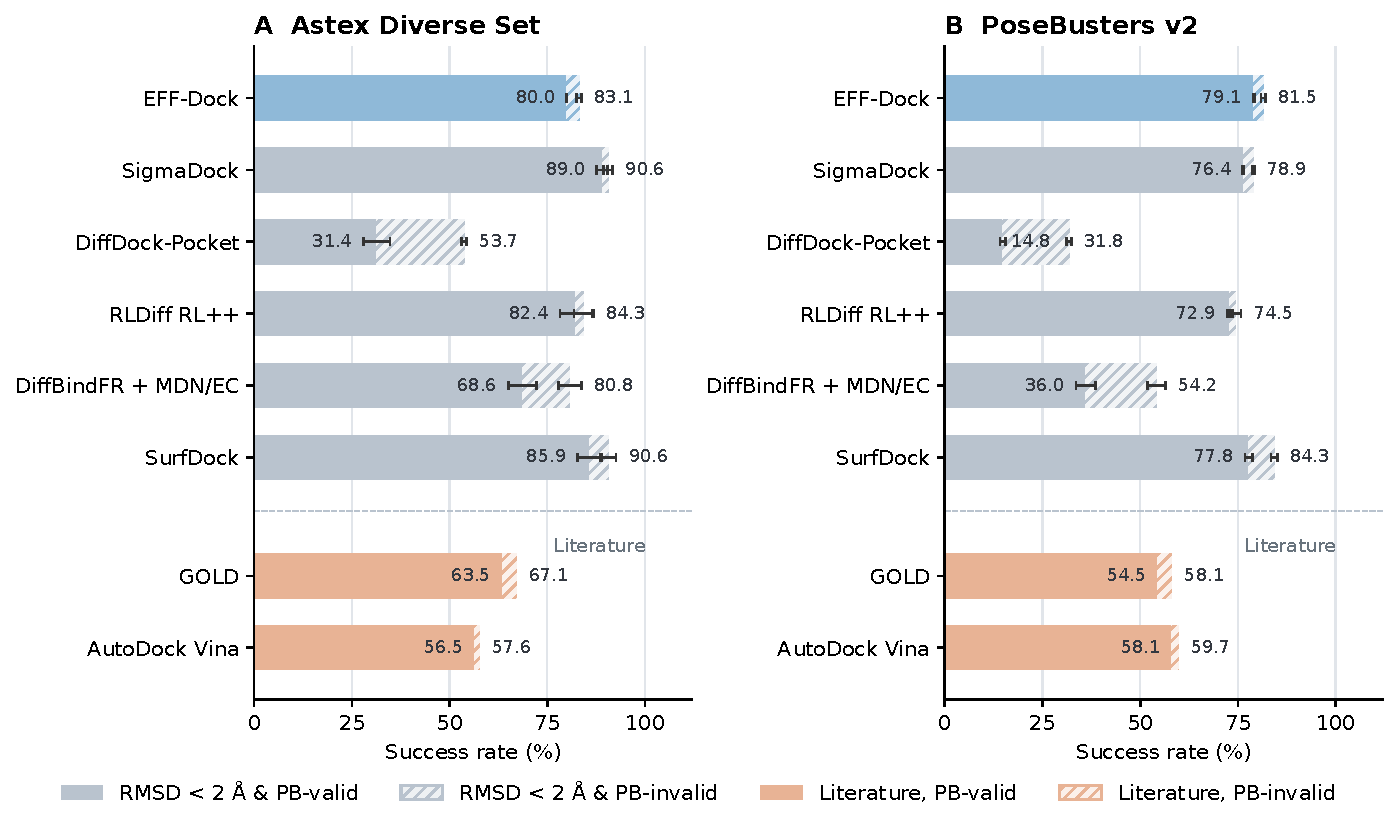
\includegraphics[width=\linewidth,height=0.68\textheight,keepaspectratio]{model_comparison.pdf}
    \caption{\textbf{External docking performance on supplied-pocket benchmarks.} (A) Astex Diverse Set (85 complexes) and (B) PoseBusters v2 (308 complexes). Solid bars show RMSD \(<2\,\angstrom\) and PoseBusters success; hatched segments complete RMSD-only success. Local results are means with sample SD across three repeats. EFF-Dock uses 100 poses, 10 sampling steps, refinement, and chirality-filtered confidence selection. GOLD and AutoDock Vina are literature values; the remaining methods use their native sampling and ranking protocols. DiffDock-Pocket uses a holo-aligned predicted receptor; DiffBindFR samples pocket side-chain torsions on a fixed backbone and uses cognate-ligand coordinates in its upstream scoring graph; its selected ligand poses are evaluated against the common frozen holo receptor. Budgets, receptor preparation, selectors and evaluation versions differ, so these are protocol-conditioned comparisons.}
    \label{fig:benchmark-comparison}
\end{figure}

\FloatBarrier

\subsection{Refinement and chirality-aware selection}

Fig.~\ref{fig:refinement-selection} compares refinement and chirality-aware selection. Refinement and rescoring increased mean RMSD--PoseBusters success by 15.7--23.2 percentage points under the primary selector and 21.7--26.5 points without chirality filtering. Without chirality filtering, mean RMSD-only selected-pose success increased more modestly. These differences combine coordinate changes with reselection and do not measure the repair of a fixed pose.

Chirality filtering added smaller mean improvements of 0.3--2.4 percentage points after refinement (Supplementary Fig.~S9). Refinement also increased input-tetrahedral compatibility across all candidate banks. Rigid fragments preserve their own geometry but do not automatically preserve stereochemistry across cut interfaces.

The complexity analysis in Supplementary Fig.~S1 localizes the remaining error.
Selected top-1 and RMSD--PoseBusters success generally deteriorated for larger ligands, more rotatable bonds, and more fragments, most clearly in PoseBusters, PhiBench-derived, and FoldBench.
Oracle success was substantially less sensitive than selected top-1, so the top-1--oracle gap tended to widen in harder strata.
Molecular complexity affects ranking and selected-pose validity as well as near-native pose generation.
The smallest Astex and high-complexity bins are too sparse for a clear trend.

\begin{figure}[!htbp]
    \centering
    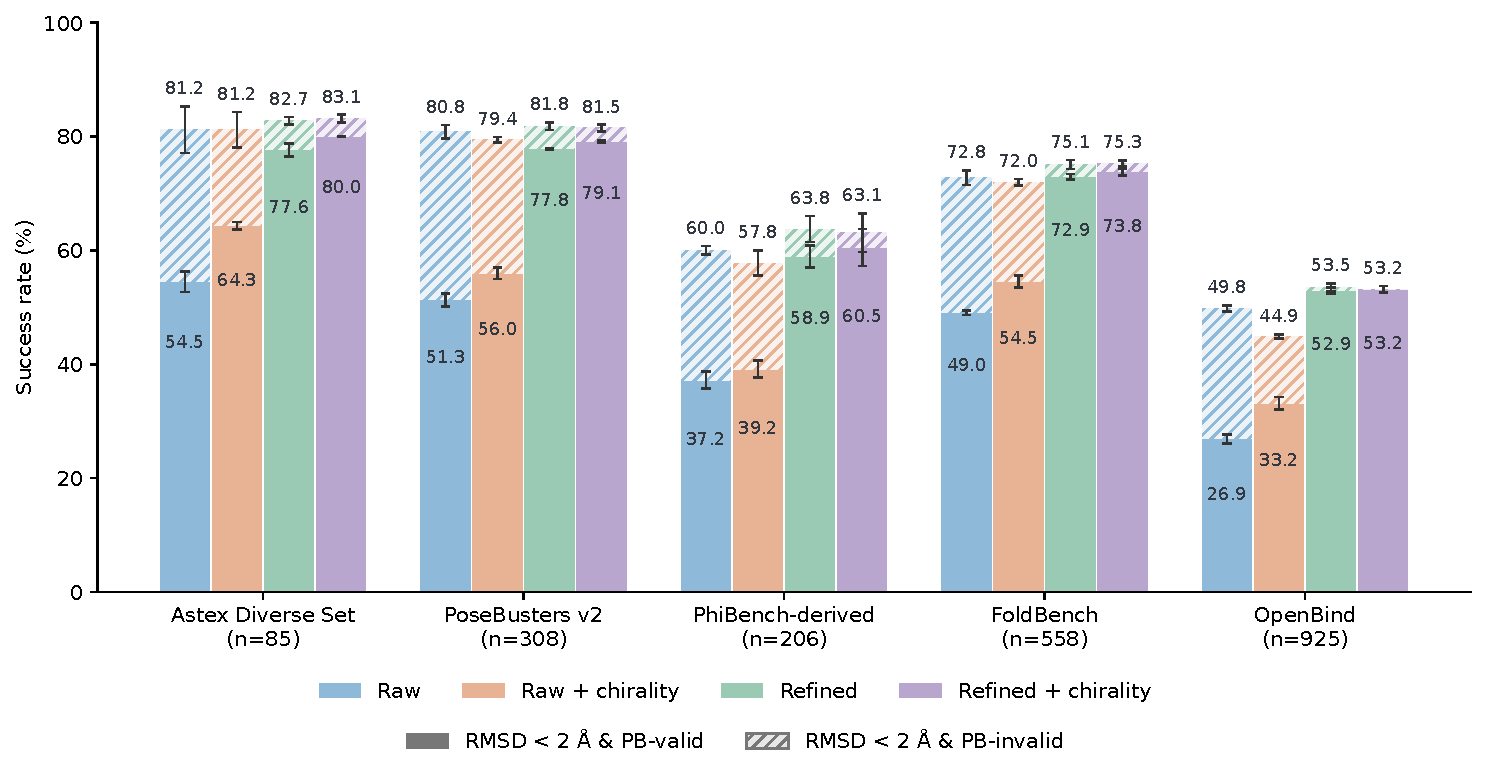
\includegraphics[width=\linewidth,height=0.68\textheight,keepaspectratio]{refinement_chirality.pdf}
    \caption{\textbf{Effects of refinement and chirality-aware selection.} \method results are shown for Astex, PoseBusters v2, PhiBench-derived, FoldBench, and OpenBind using the frozen released weights and unguided 100-pose, 10-step sampling. Raw and refined banks are ranked with or without the chirality filter. Solid bars show RMSD and PoseBusters success; hatched segments complete RMSD-only success. Bars and error bars are the mean and sample SD across three repeats on fixed cohorts.}
    \label{fig:refinement-selection}
\end{figure}

Supplementary Fig.~S16 resolves the aggregate validity gain into individual PoseBusters checks.
Refinement reduced selected-pose failures associated with bond geometry, internal clashes, receptor clashes, and internal energy, while stereochemical and ring-planarity failures were less uniformly affected.
The matched-candidate panels separate same-index fail-to-pass and pass-to-fail transitions from changes caused by selecting a different pose after refinement.
Because matched pairs exist only for candidates with saved official evaluations at both stages, these transitions diagnose the evaluated subset rather than the complete candidate banks.

\FloatBarrier

\subsection{Confidence ranking and selection headroom}

Fig.~\ref{fig:confidence-diagnostics} evaluates the ranker within each generated bank.
For refined banks, mean within-complex Spearman correlation between predicted and observed RMSD ranged from 0.51 to 0.70; near-native classification AUROC ranged from 0.88 to 0.94 and average precision from 0.61 to 0.82.
The median selection regret and conditional top-1 success in Fig.~\ref{fig:confidence-diagnostics}C,D quantify how an available RMSD-successful candidate can fail to be selected.
Reliability curves and performance as a function of near-native candidate density are reported in Supplementary Fig.~S12.

Confidence ranking enriches near-native poses at early ranks relative to generation order (Supplementary Fig.~S2). In refined unfiltered banks, expanding from top-1 to top-5 increased RMSD coverage by 7.5--20.3 percentage points, although substantial gaps to the full-bank oracle remained (Supplementary Fig.~S10). OpenBind illustrates this selection bottleneck: only 6.3\% of its refined candidates were near-native, yet 87.9\% of complexes contained at least one such pose.

The generation-prefix experiment in Supplementary Fig.~S3 reaches the same conclusion from a deployable selection perspective.
Oracle coverage cannot decrease as additional generated poses become available, whereas confidence-selected top-1 can plateau or decline when a newly added pose is incorrectly promoted.
Chirality filtering improves some prefixes but does not remove this non-monotonicity.
Larger candidate banks improve coverage, but the gain reaches top-1 only when the ranker remains stable as new poses are added.

\begin{figure}[!htbp]
    \centering
    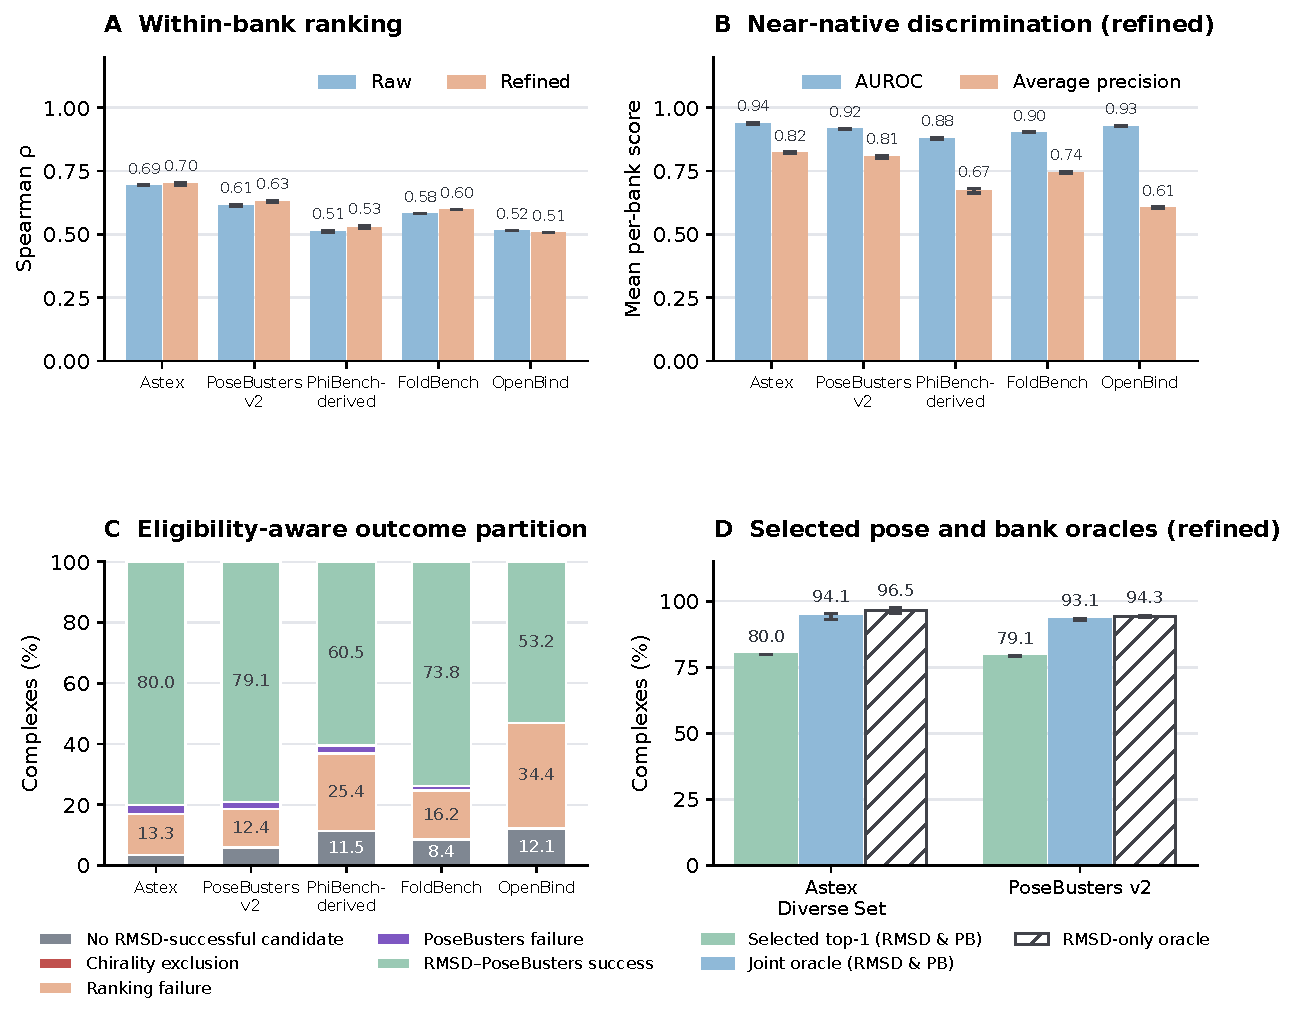
\includegraphics[width=\linewidth,height=0.70\textheight,keepaspectratio]{confidence_diagnostics.pdf}
    \caption{\textbf{Confidence ranking and remaining selection loss.} (A) Within-complex Spearman correlation between predicted and observed RMSD for raw and refined banks. (B) Refined-bank AUROC and average precision for strict RMSD \(<2\,\angstrom\) labels; single-class banks are excluded. (C) Median selected-minus-full-oracle RMSD regret. (D) Selected top-1 success conditional on the full bank containing a near-native candidate. Panels C and D use the primary chirality-filtered selector, so their loss can include eligibility exclusions. Bars show three-repeat means and sample SD.}
    \label{fig:confidence-diagnostics}
\end{figure}

\FloatBarrier

\subsection{Eligibility-aware selection bottlenecks}

Supplementary Fig.~S18 partitions every primary outcome into absence of an RMSD-successful candidate in the refined bank, exclusion of all near-native candidates by the effective chirality mask, ranking failure within the eligible set, PoseBusters failure of an RMSD-successful selection, or RMSD--PoseBusters success.
Chirality exclusion accounted for at most 0.3\% of complexes.
Ranking failure was larger, ranging from 12.4\% on PoseBusters to 34.4\% on OpenBind.
Within the refined banks, RMSD-based ranking failure exceeds chirality exclusion. Because PoseBusters was not evaluated for every candidate, this gap does not quantify attainable improvement in RMSD--PoseBusters success.
The regret curves in Supplementary Fig.~S18B measure loss relative to the best RMSD in the same effective candidate set available to the deployed selector.

Training-set relatedness is examined in Supplementary Figs.~S6--S8.
Sequence and ligand overlap differed substantially among cohorts, but neither exact ligand matches nor sequence-identity strata showed a consistent association with docking success.
These analyses qualify claims of prospective generalization without identifying a single overlap measure that explains the benchmark results.

\subsection{Sensitivity to generation inputs}

We varied the generation crop, supplied-center error and translation-prior scale on all Astex and PoseBusters complexes while holding the networks, downstream spatial context and primary selector fixed (Fig.~\ref{fig:pocket-sensitivity}). With a \(10\,\angstrom\) crop and prior scale \(2\,\angstrom\), RMSD--PoseBusters success was 80.0\% on Astex and 79.1\% on PoseBusters without center error. Center error with standard deviation \(2\,\angstrom\) per axis reduced success to 71.0\% and 64.4\%, respectively. Refined-bank RMSD-only oracle coverage at \(2\,\angstrom\) error was 86.3\% and 82.8\%.

Larger generation crops partly buffered center error, whereas prior-scale effects varied with the cohort and perturbation level. The complete crop and prior grids are shown in Fig.~\ref{fig:pocket-sensitivity}; these descriptive comparisons did not select a new operating point.

Refinement and confidence scoring retained the original unperturbed center and a \(10\,\angstrom\) crop in all conditions. The crop and center-jitter grids perturb sampling inputs with fixed downstream spatial context. Prior-scale comparisons include the scale's influence on both sampling and the recomputed docking features used for ranking. Guidance and candidate-allocation controls at equal learned pose-step counts are reported separately (Supplementary Fig.~S19).

\begin{figure}[!htbp]
    \centering
    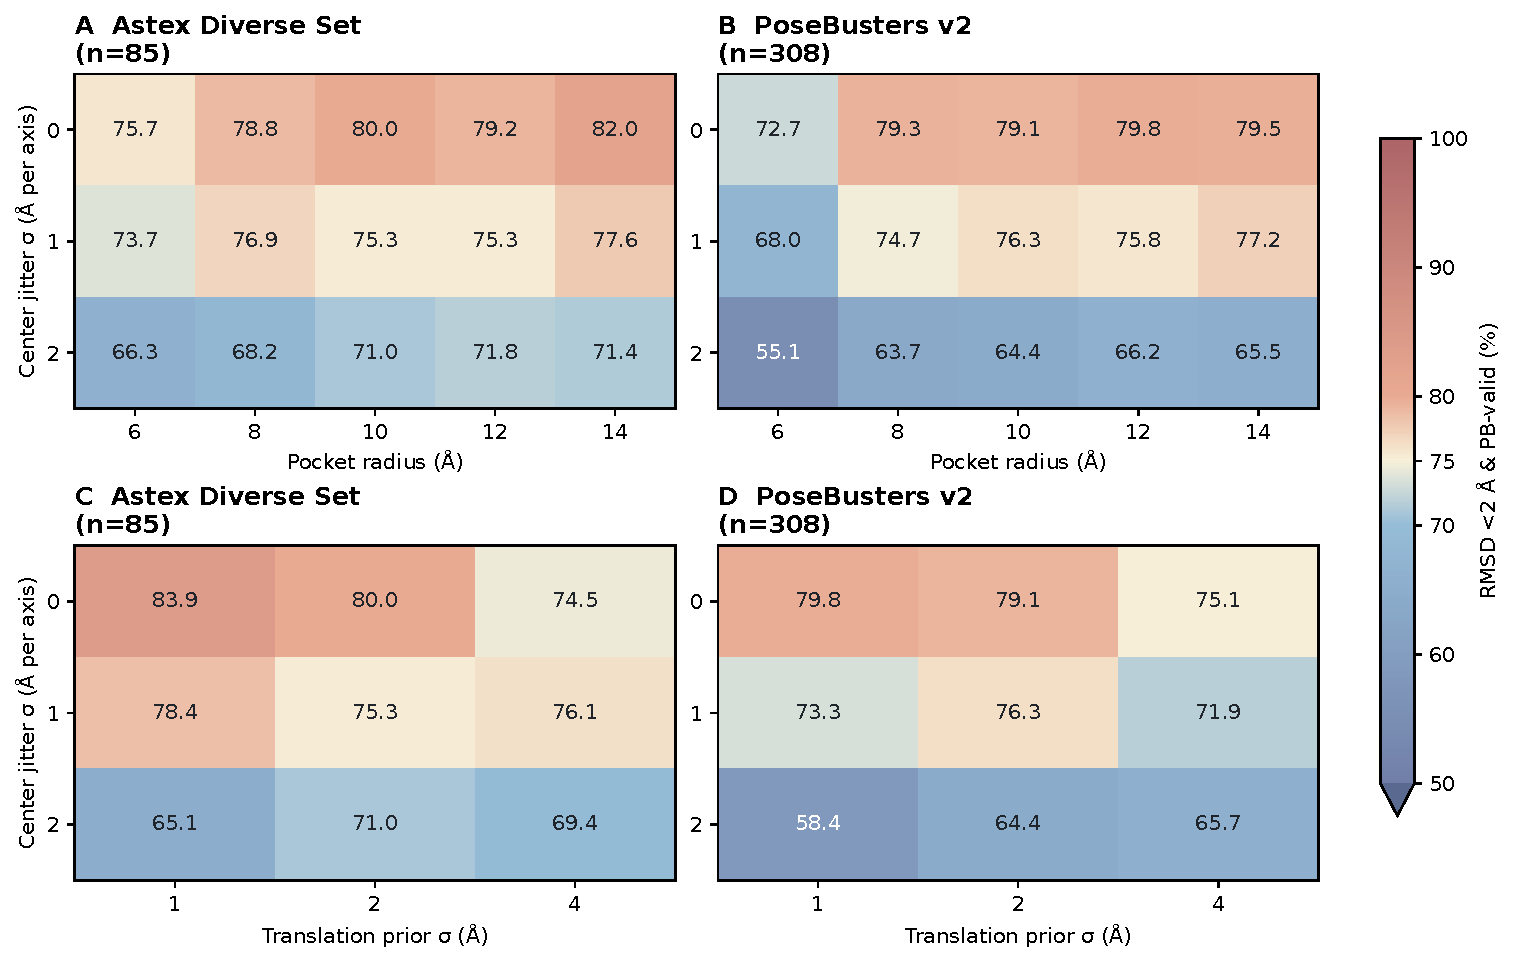
\includegraphics[width=\linewidth,height=0.78\textheight,keepaspectratio]{pocket_prior.pdf}
    \caption{\textbf{Sensitivity to supplied-pocket radius, center error and translation-prior scale.} (A,B) Joint selected-pose RMSD \(<2\,\angstrom\) and PoseBusters success across generation crop radii at prior scale \(2\,\angstrom\), for Astex Diverse Set (85 complexes) and PoseBusters v2 (308 complexes). (C,D) Prior-scale dependence at a \(10\,\angstrom\) generation crop on the same cohorts. Rows vary Gaussian center error, with standard deviation reported per Cartesian axis. Cells show three-inference-seed means. All conditions use unguided 100-pose, ten-step generation, energy refinement and chirality-filtered confidence ranking. Refinement and ranking retain the original center and \(10\,\angstrom\) crop; terminal docking features used for confidence retain the generation prior scale. The grid isolates the crop and prior axes rather than crossing every pair. Downstream spatial context is fixed; prior-scale effects include sampling and terminal feature extraction.}
    \label{fig:pocket-sensitivity}
\end{figure}

\FloatBarrier

\clearpage
\section{Discussion}
\label{sec:discussion}

The results identify coordinate validity and pose selection as distinct limitations. Refinement and rescoring increased RMSD--PoseBusters success substantially, while the smaller change in RMSD-only success indicates that geometric validity accounts for much of the gain. Matched-candidate analyses support coordinate repair, whereas aggregate gains also include reselection. The remaining RMSD-only oracle--top-1 gap identifies ranking loss without establishing that every unselected near-native pose is physically valid.

Candidate density helps explain differences among cohorts. OpenBind combined sparse near-native candidates with high full-bank coverage. Sparse banks and complex ligands were more susceptible to ranking loss, and adding candidates could reduce top-1 accuracy when an incorrect pose was promoted. The eligibility-aware analysis confirms that ranking loss was larger than chirality exclusion (Supplementary Fig.~S18).

Training relatedness showed no consistent monotonic association with success across cohorts. However, cohort composition, sparse strata and incomplete ancestral training-exposure records limit what these descriptive comparisons can establish.

\method assumes a prepared fixed receptor, one ligand chemical state and conformer, and a supplied pocket center. Receptor flexibility, pocket discovery, water rearrangement, ligand-state enumeration and covalent docking remain outside the evaluated scope. Support for selected monatomic metals does not establish general coordination-chemistry modeling. Unsupported cofactors, metal clusters and macrocycles near the fragmentation boundary also remain outside the demonstrated scope.

Training pocket centers and fragment templates were derived from crystal complexes. The center-perturbation experiments kept downstream refinement and ranking context fixed, so they do not establish complete-pipeline wrong-pocket robustness. Starting-conformer sensitivity was not systematically evaluated, and rigid-fragment motion cannot repair intrafragment errors. Fragmentation depends on atom order and uses soft cut-bond closure constraints.

The cohorts are reference-pocket redocking sets rather than prospective target-discovery benchmarks. Astex and PoseBusters were repeatedly used during development, PhiBench-derived and FoldBench adapt their source tasks, and OpenBind samples one protease family and includes two noncovalent approximations of covalent systems. Training relatedness remains substantial: all OpenBind complexes occupy the highest sequence-identity bin, and many FoldBench complexes share a training PDB accession (Supplementary Figs.~S6--S8 and Table~S16). Accession sharing does not imply the same protein--ligand complex. Only 22 external complexes met the simultaneous sequence-identity, ligand-similarity and exact-match restrictions. These evaluations therefore provide limited evidence for generalization to unrelated targets.

Component ablations are needed to distinguish the contributions of fragmentation, higher-order features, Newton--Euler readout, auxiliary losses and dynamic contacts. Confidence diagnostics quantify ranking and empirical reliability within the evaluated banks, without establishing calibration for new candidate-generation distributions. The three inference repeats describe stochastic variation under fixed trained weights, rather than retraining variability or target-population uncertainty.

Evaluation changes coordinate-to-feature handling under fixed trained weights (Supplementary Information, Secs.~S1.2--S1.3). Finite tests support covariance conditional on a fixed prepared body-coordinate convention, but do not establish invariance to supplied-conformer reorientation or unobservable fragment twist, or exact equivariance of the complete pipeline.

The interaction energy is a geometric refinement model, and the confidence score ranks poses within a candidate bank; neither predicts binding free energy or affinity. RMSD and PoseBusters assess pose accuracy and common coordinate errors, but do not establish binding or identify every valid binding mode.

\method combines rigid-fragment flow matching with geometric refinement and confidence ranking. The evaluated 100-pose protocol provides high near-native coverage, while the remaining selection loss motivates better ranking and broader validation of receptor and ligand preparation.

\section{Online Methods}\label{sec:online-methods}
\label{sec:method}

\subsection{Coordinate convention and evaluated weights}
\label{sec:orientation_convention}

The coordinate reconstruction in Eq.~\eqref{eq:pose_manifold} uses an active local-to-world rotation, \(\mathbf x=\mathbf R\mathbf y+\mathbf T\).
Equivariance is defined conditional on a fixed prepared fragment-local template and its body-coordinate convention. Under a joint rigid transformation of the receptor and current ligand pose, the prepared local coordinates remain fixed while world coordinates transform as \(\mathbf x'=\mathbf Q\mathbf x+\mathbf a\) and fragment rotations as \(\mathbf R'=\mathbf Q\mathbf R\). Supplied conformers are centered fragment-wise without canonicalizing their local axes.
Accordingly, a learned fragment-local vector \(\mathbf w\) is injected into world-frame features as
\begin{equation}
    \mathbf h=\mathbf R\mathbf w,
    \qquad
    \mathbf h'=(\mathbf Q\mathbf R)\mathbf w=\mathbf Q\mathbf h
    \label{eq:orientation_injection}
\end{equation}
under a joint world rotation \(\mathbf Q\in\SO(3)\).
Source-local edge coordinates of the form \(\mathbf R^\top(\mathbf x_j-\mathbf x_i)\) perform the inverse world-to-local map.

All measurements use fixed docking and confidence weights; no retraining, probability recalibration, or result-dependent thresholding was performed.
Coordinate-to-feature conventions, their differences from training, and finite numerical verification are documented in the \sisection{S1.2}.

\subsection{Task definition and fragment pose representation}
\label{sec:problem}

\method takes a prepared fixed receptor \(\mathcal{P}\), a heavy-atom ligand graph \(\mathcal{G}_{L}\) in one specified chemical state, one supplied or generated ligand conformer \(\mathcal{C}_{L}\), and an explicit pocket center \(\mathbf{b}\in\R^3\).
We denote their complete conditioning context by \(\mathcal{C}_{\mathrm{cond}}=(\mathcal{P},\mathcal{G}_{L},\mathcal{C}_{L},\mathbf{b})\).
It returns a finite set of ligand poses and a separate score used only to rank poses within that set.
Target ligand coordinates, target-derived atom or fragment frames, RMSD, validity outcomes, and benchmark identity are excluded from deployment inputs.
Reference-derived pocket centers are used only in experiments explicitly labelled reference-pocket redocking and are not interpreted as pocket discovery.

The ligand contains \(N\) heavy atoms partitioned into \(K\) rigid fragments, with \(i\in\{1,\ldots,N\}\) and \(k\in\{1,\ldots,K\}\) indexing atoms and fragments, respectively.
The map \(g(i)\) assigns atom \(i\) to a fragment, and \(\mathbf{y}_i\in\R^3\) is its local coordinate relative to that fragment's geometric centroid.
The generative state and atom reconstruction are
\begin{equation}
    \mathcal{M}_{L}
    =
    \prod_{k=1}^{K}\left(\R^3\times\SO(3)\right),
    \qquad
    \mathbf{z}
    =
    \{(\mathbf{T}_k,\mathbf{R}_k)\}_{k=1}^{K},
    \qquad
    \mathbf{x}_i(\mathbf{z})
    =
    \mathbf{R}_{g(i)}\mathbf{y}_i+\mathbf{T}_{g(i)}.
    \label{eq:pose_manifold}
\end{equation}
Here \(\mathcal{M}_{L}\) is the ligand pose space, \(\R^3\) is the translation space, and \(\SO(3)\) is the group of proper three-dimensional rotations.
For fragment \(k\), \(\mathbf{T}_k\in\R^3\) is its geometric-centroid state origin and \(\mathbf{R}_k\in\SO(3)\) is its rotation; \(\mathbf{z}\) collects all fragment states, and \(\mathbf{x}_i(\mathbf{z})\in\R^3\) is the reconstructed coordinate of ligand atom \(i\) in the pocket-centered frame.
This representation preserves intrafragment geometry while allowing fragments to translate and rotate relative to one another.

Ligands are standardized with RDKit \citep{landrum2024rdkit}: stereochemistry is assigned before hydrogen removal, the largest connected component is retained, and formal charge and the supplied protonation state are preserved.
For simplified molecular-input line-entry system (SMILES) input, the inference path constructs one seeded Experimental-Torsion Knowledge Distance Geometry version 3 (ETKDGv3) conformer \citep{wang2020etkdgv3}, followed by at most 200 Merck Molecular Force Field (MMFF) iterations \citep{halgren1996mmff}; supplied structure-data file (SDF) or Tripos MOL2 coordinates are retained.
The receptor is hydrogen-stripped and fixed, and all receptor and ligand coordinates are translated by \(-\mathbf{b}\) so that the supplied pocket center is the origin.
For geometry training, each deposited crystal ligand pose is fragmented in its bound conformation, and the resulting crystal coordinates define the fixed fragment-local coordinates used as model input and reconstruction templates.
Prospective inputs instead use supplied or independently generated conformers; rigid-fragment motion cannot correct internal differences within a fragment.
Exact input normalization and pocket provenance are given in the \sisection{S1}.

\subsection{Fragmentation and pocket-conditioned graph}
\label{sec:fragmentation}
\label{sec:graph}

Fragmentation cuts eligible heavy-atom single bonds outside rings while excluding planar carbonyl C--N/O and sulfonyl S--N linkages.
Connected components define provisional rigid fragments, singleton components are merged into adjacent fragments, and the retained cut topology supplies fragment adjacency and local cross-fragment distance constraints.
This indexed greedy rule is deterministic for a fixed atom ordering; exact eligibility, tie-breaking, and failure handling are specified in the \sisection{S2.1}.

The receptor is cropped residue-wise around the supplied center.
Geometry training samples a radius uniformly from \(6\) to \(12\,\angstrom\) and applies isotropic center jitter with standard deviation \(2\,\angstrom\); held-out validation uses an \(8\,\angstrom\) crop, and the external reference-pocket protocol uses a fixed \(10\,\angstrom\) crop.
The graph contains ligand atoms, ligand fragments, protein atoms, and residue virtual nodes.
Typed static relations encode covalent structure, fragment membership and topology, protein hierarchy, and residue--fragment context, while protein-atom--ligand-atom contacts within \(5\,\angstrom\) are rebuilt at every forward pass.
Node chemistry, all ten directed relation types, crop fallbacks, and edge descriptors are listed in the \sisection{S3.1}.

\subsection{Equivariant fragment flow and Newton--Euler readout}
\label{sec:flow}

After pocket centering, fragment translations are drawn from an isotropic Gaussian and multi-atom fragment rotations from the uniform distribution on \(\SO(3)\) \citep{shoemake1992uniform}.
Let \(t\in[0,1]\) denote dimensionless flow time, with subscripts \(0\) and \(1\) denoting the sampled prior and bound target states, respectively, and let \(\sigma>0\) be the translation-prior standard deviation in Angstrom.
For a paired prior and target state, translations follow a linear path and rotations follow the shortest geodesic under a left-action convention:
\begin{align}
    \mathbf{T}_{k,0}
    &\sim\mathcal{N}(\mathbf{0},\sigma^2\mathbf{I}_3),
    &
    \mathbf{R}_{k,0}
    &\sim\mathrm{Uniform}(\SO(3)),
    \nonumber\\
    \mathbf{T}_{k,t}
    &=(1-t)\mathbf{T}_{k,0}+t\mathbf{T}_{k,1},
    &
    \mathbf{R}_{k,t}
    &=\operatorname{Exp}(t\boldsymbol{\omega}^{\star}_k)\mathbf{R}_{k,0},
    \nonumber\\
    \mathbf{v}^{\star}_k
    &=\mathbf{T}_{k,1}-\mathbf{T}_{k,0},
    &
    \boldsymbol{\omega}^{\star}_k
    &=\operatorname{Log}(\mathbf{R}_{k,1}\mathbf{R}_{k,0}^{-1}).
    \label{eq:flow_path}
\end{align}
Here \(\mathcal{N}(\mathbf{0},\sigma^2\mathbf{I}_3)\) is the three-dimensional Gaussian prior and \(\mathrm{Uniform}(\SO(3))\) is the normalized Haar distribution over rotations.
The maps \(\operatorname{Exp}:\R^3\rightarrow\SO(3)\) and \(\operatorname{Log}:\SO(3)\rightarrow\R^3\) are the rotation exponential and principal logarithm under the axis--angle identification.
The starred vectors \(\mathbf{v}^{\star}_k\) and \(\boldsymbol{\omega}^{\star}_k\) are the target translational and angular tangents, measured in Angstrom and radians per unit flow time, respectively.
Singleton rotations are fixed to identity and contribute no supervised angular mode.
At time \(t\), \(\mathbf{z}_t=\{(\mathbf{T}_{k,t},\mathbf{R}_{k,t})\}_{k=1}^{K}\) denotes the interpolated ligand state.
Conditional flow matching trains the vector field \(u_{\theta}(\mathbf{z}_t,t,\mathcal{C}_{\mathrm{cond}},\sigma)\), with learned parameters \(\theta\), to return the fragment-wise predictions \(\{(\widehat{\mathbf{v}}_k,\widehat{\boldsymbol{\omega}}_k)\}_{k=1}^{K}\) and match the starred targets without integrating the generative ODE during training \citep{lipman2023flow}.
The prior-scale mixture, time distribution, rotation augmentation, and numerical path conventions are recorded in the \sisection{S2}.

\paragraph{Equivariant trunk and Newton--Euler readout.}
\label{sec:equivariant_network}
\label{sec:newton_euler}

All node types share six equivariant interaction layers with 384 scalar channels, 32 channels of each vector parity and 16 channels of each rank-two parity. Time and prior scale enter through a 128-dimensional conditioning embedding. Each layer combines normalized sender features, radial edge features and real spherical harmonics through order two using tensor products, gated residual aggregation and adaptive normalization. Static relations and rebuilt protein--ligand contacts use relation-specific edge features. Complete equations and dimensions are given in the \sisection{S3}.

The output head predicts one polar atom-vector proposal \(\mathbf{f}_i\) for each ligand atom. Its unit-weight Newton--Euler aggregation is a least-squares rigid-body velocity fit restricted to the retained rotational modes; these vectors are not physical forces or energy gradients.
For fragment \(k\), with atom set \(\mathcal{A}_k\), center \(\mathbf{T}_k\), and lever arm \(\mathbf{r}_i=\mathbf{x}_i-\mathbf{T}_k\), the fragment field is obtained by
\begin{align}
    \widehat{\mathbf{v}}_k
    &=
    \frac{1}{|\mathcal{A}_k|}
    \sum_{i\in\mathcal{A}_k}\mathbf{f}_i,
    &
    \boldsymbol{\mu}_k
    &=
    \sum_{i\in\mathcal{A}_k}\mathbf{r}_i\times\mathbf{f}_i,
    \nonumber\\
    \mathbf{J}_k
    &=
    \sum_{i\in\mathcal{A}_k}
    \left(
      \|\mathbf{r}_i\|_2^2\mathbf{I}_3
      -\mathbf{r}_i\mathbf{r}_i^{\top}
    \right),
    &
    \widehat{\boldsymbol{\omega}}_k
    &=\mathbf{J}_k^{+}\boldsymbol{\mu}_k.
    \label{eq:newton_euler}
\end{align}
Here \(\widehat{\mathbf{v}}_k\) is the predicted translational tangent, \(\boldsymbol{\mu}_k\) is the moment of the atom vectors, \(\mathbf{J}_k\) is the unit-mass geometric inertia about the fragment centroid, and \(\widehat{\boldsymbol{\omega}}_k\) is the predicted angular tangent.
The truncated pseudoinverse \(\mathbf{J}_k^+\) removes geometric-inertia eigenmodes at or below 1\% of the largest eigenvalue, and the same observable subspace is applied to the angular training target.
This prevents singleton and nearly collinear fragments from receiving arbitrary angular velocities; the exact eigenspace construction is given in the \sisection{S3.2}.

\subsection{Objective and sampling}
\label{sec:objective}
\label{sec:sampling}

The primary losses are mean-squared errors (MSEs) on fragment translation and observable angular velocity.
The geometry objective combines fragment translation and observable angular-velocity errors with two auxiliary terms:
\begin{equation}
    \mathcal{L}_{\mathrm{geom}}
    =\mathcal{L}_{v}
     +\lambda_{\omega}\mathcal{L}_{\omega}
     +\lambda_{\mathrm{atom}}\mathcal{L}_{\mathrm{atom}}
     +\lambda_{\mathrm{DG}}\mathcal{L}_{\mathrm{DG}}.
    \label{eq:geometry_objective}
\end{equation}
Here \(\mathcal L_v\) is fragment translation MSE, \(\mathcal L_\omega\) is angular MSE after projecting the target onto retained rotational modes, and \(\mathcal L_{\mathrm{atom}}\) compares reconstructed atom velocities. The distance-geometry term \(\mathcal L_{\mathrm{DG}}\) compares interfragment atom-pair distances after a one-step endpoint extrapolation, with a \(t^2\)-weighted valid-complex reduction. Unobservable terms contribute zero. The final continuation uses weights \((\lambda_\omega,\lambda_{\mathrm{atom}},\lambda_{\mathrm{DG}})=(8,0.3,3)\); definitions, normalizations and distributed reductions are given in the \sisection{S3.3}.

The final continuation samples flow time from an 80\% base distribution, a 10\% uniform component on \([0,0.3]\), and a 10\% point mass at \(t=0\). The base distribution mixes uniform sampling with a late-biased logit-normal distribution. Its parameters and the prior-scale mixture are specified in the \sisection{S2}.

At inference, sampled fragment priors are integrated from \(t=0\) to \(1\) using 10 late-biased Euler intervals in the primary protocol.
For interval width \(\Delta t\), translations receive additive increments and rotations are advanced by left multiplication with \(\operatorname{Exp}(\Delta t\,\widetilde{\boldsymbol{\omega}}_k)\), where the tilde denotes the guided field when guidance is enabled.
Atom coordinates and dynamic protein--ligand contacts are rebuilt before every field evaluation.
The sampling schedule and candidate selection are specified in the \sisection{S2.2}.

\subsection{Confidence-based pose selection}
\label{sec:confidence}

Pose generation and top-1 selection are separated.
For each candidate, the fixed docking network is evaluated at \(t=1\), using recovered fragment frames and the source translation-prior scale, to recompute terminal ligand representations. A second equivariant network combines these with a fresh heterogeneous-graph embedding and applies four additional interaction layers.
Invariantized node features and explicit protein-contact summaries are pooled by ligand-contact attention and type-wise mean--maximum aggregation.
Atom and pose heads are trained with displacement and RMSD regression, \(2\,\angstrom\) success classification, pairwise ranking, and a success-focused listwise objective.
For a candidate set \(\{\mathbf z_S^{(m)}\}_{m=1}^{M}\), the deployed selector is
\begin{equation}
    \mathcal E=\begin{cases}
       \{m:q_m=1\}, & \text{if any }q_m=1,\\
       \{1,\ldots,M\}, & \text{otherwise},
    \end{cases}
    \qquad
    m^\star=\operatorname*{arg\,min}_{m\in\mathcal E}
    c_\phi\!\left(\mathbf z_S^{(m)},\mathcal P,\mathcal G_L,\mathcal C_L,\sigma\right).
    \label{eq:confidence_selection}
\end{equation}
Here \(q_m\) denotes compatibility with the input-defined tetrahedral stereocenters. Ties follow saved candidate order. The unfiltered argmin is reported separately as a diagnostic condition.
The confidence network's nonnegative predicted-RMSD score is \(c_\phi\), with learned parameters \(\phi\); \(m^\star\) is the selected candidate index.
The prior scale enters this score through the recomputed docking representations.
The score is interpreted only as a within-candidate-set ranking signal and not as calibrated RMSD, uncertainty, binding probability, or affinity.
Energy restraints and confidence features use conformers prepared by the same procedure and seed as pose generation. Refinement preserves each saved candidate's fragment-internal coordinates. For rescoring, candidate coordinates are mapped to fragment frames by proper Kabsch fitting for templates of rank at least two and an input-indexed, scene-defined convention for lower-rank fragments. This resolves the recovery convention without making the frozen network invariant to unobservable fragment twist; finite numerical checks and their limits are reported in the \sisection{S1.3}.
The complete readout and confidence objective are given in the \sisection{S4}.

\FloatBarrier

\subsection{Differentiable guidance and post-sampling refinement}
\label{sec:guidance}

For ligand coordinates \(\mathbf{x}=(\mathbf{x}_1,\ldots,\mathbf{x}_N)\), we define a differentiable guidance energy
\begin{align}
    E_{\mathrm{G}}&=E_{\mathrm{phys}}+E_{\mathrm{int}},\nonumber\\
    E_{\mathrm{phys}}&=E_{\mathrm{bond}}+E_{\mathrm{angle}}+E_{\mathrm{proper}}
      +E_{\mathrm{chiral}}+E_{\mathrm{planar}}\nonumber\\
      &\quad+E_{\mathrm{LJ}}+E_{\mathrm{steric}}+E_{\mathrm{obs}},\nonumber\\
    E_{\mathrm{int}}&=E_{\mathrm{hyd}}+E_{\mathrm{HB}}+E_{\mathrm{chg}}
      +E_{\pi}+E_{\mathrm{cat}\text{-}\pi}+E_{\mathrm{XB}}+E_{\mathrm{metal}}.
    \label{eq:guidance_total}
\end{align}
The cut-interface terms restrain only bond, angle, proper-torsion, chiral, and planar geometry that spans independently moving fragments.
The nonbonded terms include a soft-core Universal Force Field (UFF)-style Lennard--Jones profile on admitted interfragment ligand--ligand and protein--ligand pairs, a compact receptor-overlap barrier and repulsion-only obstacles for unresolved receptor chemistry \citep{rappe1992uff}.
The seven interaction terms describe hydrophobic contacts, directional hydrogen bonds, screened formal-charge groups, pi stacking, cation--pi contacts, halogen bonds, and typed metal coordination \citep{salentin2015plip,mcgaughey1998pistacking,gallivan1999cationpi,desiraju2013halogen,dokmanic2008metals}.
These bounded geometric preferences do not define binding free energy, affinity, or a molecular-dynamics Hamiltonian.

Compact radial and angular gates use a clipped quintic smoothstep with zero first and second derivatives at its endpoints. This cutoff envelope joins constant regions with continuous energy and first and second derivatives; it is not a physical force law. Energy forms, occupancy aggregation, typing conventions and numerical constants are specified in the \sisection{S5}.

The coordinate gradient \(\nabla_{\mathbf{x}_i}\) gives the guidance force \(\mathbf{F}_i=-\nabla_{\mathbf{x}_i}E_{\mathrm{G}}\), which is distinct from the learned atom-vector proposal \(\mathbf{f}_i\).
For atom mass \(m_i\), the fragment mass is \(m_k^{\mathrm{frag}}=\sum_{i\in\mathcal{A}_k}m_i\), the center of mass is \(\mathbf{c}_k=(m_k^{\mathrm{frag}})^{-1}\sum_{i\in\mathcal{A}_k}m_i\mathbf{x}_i\), and the resultant is \(\mathbf{F}_k=\sum_{i\in\mathcal{A}_k}\mathbf{F}_i\).
The vector \(\boldsymbol{\tau}_k=\sum_{i\in\mathcal{A}_k}(\mathbf{x}_i-\mathbf{c}_k)\times\mathbf{F}_i\) is the center-of-mass torque, and \(\mathbf{I}_k\) is the corresponding mass-weighted inertia tensor.
The translational and angular guidance directions are
\begin{equation}
    \mathbf{d}^{\omega}_k
    =\mathbf{I}_k^{+}\boldsymbol{\tau}_k,
    \qquad
    \mathbf{d}^{T}_k
    =\frac{\mathbf{F}_k}{m_k^{\mathrm{frag}}}
     +\mathbf{d}^{\omega}_k\times(\mathbf{T}_k-\mathbf{c}_k).
    \label{eq:guidance_projection}
\end{equation}
Here \(\mathbf{d}^{T}_k\) and \(\mathbf{d}^{\omega}_k\) are guidance directions, \(\mathbf{I}_k^+\) is the mass-inertia truncated pseudoinverse, and \(\mathbf{T}_k-\mathbf{c}_k\) corrects for the offset between the fragment's geometric-centroid state origin and its center of mass.
For guidance experiments, let \((\Delta\mathbf v_k,\Delta\boldsymbol\omega_k)\) denote the mass--inertia directions after RMS matching to the learned atom velocity, late-time interval ramping, and the translation, rotation, and atom-displacement caps.  The guided field is
\begin{equation}
    \widetilde{\mathbf v}_k
    =\widehat{\mathbf v}_k+\Delta\mathbf v_k,
    \qquad
    \widetilde{\boldsymbol\omega}_k
    =\widehat{\boldsymbol\omega}_k+\Delta\boldsymbol\omega_k,
    \label{eq:guidance_drift}
\end{equation}
where \(\eta\) controls the pre-cap guidance strength; the exact interval average, normalization, zero-direction rule, and caps are given in the \sisection{S5.9}.
This inference-time modification is conceptually related to guidance of flow-matching vector fields, although the normalization and fragment projection used here are method specific \citep{feng2025flowguidance}.
Post-sampling refinement updates only the fragment state of each candidate.  At refinement iteration \(r\),
\begin{equation}
    \mathbf{T}_k^{(r+1)}
    =\mathbf{T}_k^{(r)}+\alpha_r\bar{\mathbf{d}}_k^T,
    \qquad
    \mathbf{R}_k^{(r+1)}
    =\operatorname{Exp}(\alpha_r\bar{\mathbf{d}}_k^\omega)
     \mathbf{R}_k^{(r)},
    \label{eq:guidance_refinement}
\end{equation}
Here \((\bar{\mathbf d}^T,\bar{\mathbf d}^\omega)=\operatorname{Cap}(\mathbf d^T,\mathbf d^\omega)\) are capped increments and \(\alpha_r\) is the accepted line-search step size. The cap first bounds each fragment translation and rotation separately, then jointly rescales both until the reconstructed atom displacement meets its bound.  Writing \(E_r=E_{\mathrm G}(\mathbf{x}^{(r)})\), the proposed translation, rotation, and induced atom displacement are bounded and \(\alpha_r\) is reduced by monotone backtracking until a finite non-increasing guidance energy is obtained.
The refinement is bounded and stops on convergence, line-search failure, or a sustained energy plateau; the numerical safeguards and termination criteria are given in the \sisection{S5.10}.
Raw and refined candidates are compared with unchanged network parameters.

The guidance subsystem uses a typed \(18\,\angstrom\) receptor shell, which can expose coordinates outside the \(10\,\angstrom\) neural crop.
This shell is not an additional neural input.
Full typing rules, energy equations, mass--inertia projection, refinement safeguards, and permitted information are provided in the \sisection{S5}.

\label{sec:experiments}

\subsection{Data curation and split}
\label{sec:data_curation}
\label{sec:split_boundary}

Training data were derived from PLINDER 2024-06/v2 \citep{durairaj2024plinder}. Curation applies ligand validity, covalency, interaction, experimental-quality, resolution, contact and size criteria, followed by deterministic representative selection within ligand and pocket-community groups. The filters and cohort counts are detailed in the \sisection{S6}.

After model-specific input filtering, docking uses 47,277 training and 1,076 validation samples, while confidence uses 43,092 training and 1,035 validation samples. Their differing input requirements and overlap are detailed in the \sisection{S6}.

External exclusion required both an exact ligand match and membership in a benchmark-associated pocket community, removing 904 samples. This rule does not independently exclude recurring ligands or homologous proteins; training relatedness is measured separately.

\subsection{Evaluation scope}
\label{sec:information_boundary}

Row-level splits can share repeated ligands or homologous proteins, so training-set relatedness is measured explicitly rather than inferred from split labels \citep{durairaj2024plinder,corso2024dockgen,morehead2026posebench,skrinjar2026generalization}.
For each external cohort, we report the receptor state, pocket source, ligand preparation, candidate budget, and selector.
Astex and PoseBusters were used during development and are treated as descriptive benchmarks.

The geometry model uses the receptor crop, ligand graph, starting conformer, pocket center, and current sampled coordinates.
The confidence model ranks the generated candidates from the same task inputs.
The interaction energy may additionally read a larger receptor shell, but it has no access to the crystal pose, RMSD, or validity labels.
Raw coordinates are saved before refinement.

\subsection{Model training and selection}
\label{sec:geometry_training}
\label{sec:confidence_training}

The docking model was trained for 200,000 base updates, 100,000 geometry-fine-tuning updates and 50,000 early-time-replay updates, with global batch sizes of 256, 256 and 64. The final stage used AdamW with peak learning rate \(2\times10^{-5}\), weight decay 0.01, gradient clipping at 1.0 and EMA decay 0.999 \citep{loshchilov2019decoupled}; its terminal EMA was evaluated. The confidence model was trained on raw and refined poses and selected at update 70,000 by predicted-RMSD-ranked top-1 success on 1,035 internal-validation complexes. Training stages, initialization, optimization schedules and selection criteria are specified in the \sisection{S6.4}. External benchmark results did not select the evaluated checkpoints.

\subsection{Benchmarks and comparison protocol}
\label{sec:evaluation_tasks}
\label{sec:baselines}

The evaluation uses five complementary cohorts.
The Astex Diverse Set contains 85 curated complexes \citep{hartshorn2007astex}, and PoseBusters v2 contains 308 complexes with detailed coordinate-validity checks \citep{buttenschoen2024posebusters}.
The PhiBench-derived cohort comprises 206 locally selected complexes from the public PhysDock archive; identity with the published 206-case cohort has not been established \citep{zhang2025physdock}.
FoldBench-Pocket contains 558 released protein--ligand interfaces, including a 66-interface post-June 2024 slice \citep{xu2026foldbench}.
OpenBind contains 925 EV-A71/CVA16 2A-protease complexes and is an auxiliary single-family cohort, including two flagged noncovalent approximations of covalent systems \citep{openbind2026eva71}.

All five cohorts are evaluated by holo-receptor, reference-pocket redocking.
The pocket center is computed from receptor residue nodes within \(8\,\angstrom\) of the reference ligand, and the reference ligand is then removed from the model input.

The primary setting uses 100 candidates, 10 late-biased Euler steps, \(\sigma=2\,\angstrom\), a \(10\,\angstrom\) receptor crop, and no inference-time guidance.
Each cohort uses the same trained weights with inference seeds 42, 100042 and 200042. Astex and PoseBusters fix the ETKDG seed at zero for generation; PhiBench-derived, FoldBench and OpenBind use the per-complex sampling seed for conformer generation, so their repeat variability also includes starting-conformer variation.
Candidates are scored before and after bounded refinement.
The primary selector removes chirality-mismatched candidates and then chooses the lowest predicted symmetry-aware RMSD; if none passes the chirality screen, it uses the unfiltered ranking.
Failed complexes remain in the cohort denominator.
Supplementary Figs.~S4 and S5 report runtime and generation-process memory for the candidate-acquisition runs, including their original refinement and confidence scoring but excluding subsequent refinement and rescoring passes. These are not end-to-end timings of the primary evaluation. Sensitivity to generation inputs is analyzed in Fig.~\ref{fig:pocket-sensitivity}; supplementary guidance controls are described below.

\subsection{Generation-input sensitivity and guidance controls}

Sensitivity experiments use all 85 Astex and 308 PoseBusters complexes with the same three inference seeds and chirality-filtered selector. At translation-prior scale \(2\,\angstrom\), generation crop radii \(6,8,10,12,14\,\angstrom\) are crossed with Gaussian center jitter of \(0,1,2\,\angstrom\) per Cartesian axis. Separately, prior scales \(1,2,4\,\angstrom\) are crossed with the same jitter levels at a \(10\,\angstrom\) crop. Shared cells are evaluated once, and the primary baseline is reused from the primary evaluation. The jitter random stream is independent of the pose prior, and matching seeds couple prior draws within a candidate budget. Refinement and confidence scoring always use the original center and a \(10\,\angstrom\) crop; the docking-feature re-evaluation used for confidence scoring retains each candidate's source prior scale.

Four budget/guidance conditions, including the shared primary baseline, cross 100 poses/ten steps or 40 poses/25 steps with unguided sampling or normalized energy guidance of strength \(\eta=2\). Both budgets use 1,000 learned pose-steps, but guidance and candidate processing add work, so equal pose-step counts do not imply equal runtime. Forty- and 100-pose banks are generated separately, without a nested-prior claim. All sensitivity and guidance conditions are descriptive external evaluations and do not choose a sampler, guidance strength or selector.

\subsection{Endpoints and statistical analysis}
\label{sec:metrics}

The primary pose endpoint is confidence-selected, symmetry-aware heavy-atom RMSD below \(2\,\angstrom\) after complete atom mapping.
Secondary endpoints include top-\(q\) and oracle-\(q\) coverage and complete-case RMSD summaries.
Physical validity uses PoseBusters 0.6.5 in \texttt{redock} mode, with a reference-molecule representation adapter for the three temporal cohorts as detailed in the \sisection{S7}; pass-all is the conjunction of all 27 non-RMSD checks on the same selected pose \citep{buttenschoen2024posebusters}.
RMSD--PoseBusters success requires both RMSD \(<2\,\angstrom\) and PoseBusters pass-all.

Binary endpoints use the full cohort denominator; continuous summaries use successfully evaluated poses and report their coverage.
Error bars are sample standard deviations across the three repeats unless stated otherwise.
Supplementary Figs.~S9 and S14 use paired 95\% bootstrap intervals.
Further evaluation details are given in the \sisection{S7}.

\subsection{Use of automated tools}

OpenAI Codex and Anthropic Claude were used to assist with code review, analysis-script development, manuscript drafting, consistency checks and language editing.
The authors reviewed the generated text against the source code and primary literature and retain full responsibility for the manuscript.
These tools are not authors.

\section*{Data and Code Availability}

Source code, model weights, training-membership lists, numerical source data and analysis scripts are available at \href{https://github.com/eightmm/EFF-Dock}{https://github.com/eightmm/EFF-Dock}. Benchmark structures remain subject to their original distribution and redistribution terms.

\section*{Author Contributions}

J.S.: conceptualization, methodology, software, validation, formal analysis, investigation, data curation, visualization, and writing---original draft.
J.L.: conceptualization, methodology, resources, supervision, project administration, and writing---review and editing.
Both authors are responsible for the final scientific content.

\section*{Competing Interests}

J.L.'s affiliation with Arontier Co. is disclosed in the author information.

\section*{Supplementary Information}

Supplementary methods and analyses are provided in the accompanying Supplementary Information.

\bibliographystyle{unsrt}
\bibliography{references}

\end{document}
